% me=0 student solutions (ps file), me=1 - my solutions (sol file),
% me=2 - assignment (hw file)
\def\me{0} \def\num{9} %homework number

\def\due{5 pm on Thursday November, 21} %due date

\def\course{CSCI-GA.1170-001/002 Fundamental Algorithms} 
%course name, changed only once

% **** INSERT YOUR NAME HERE ****
\def\name{jingshuai jiang}

% **** INSERT YOUR NETID HERE ****
\def\netid{jj2903}

% **** INSERT NETIDs OF YOUR COLLABORATORS HERE ****
\def\collabs{NetID1, NetID2}


\iffalse

INSTRUCTIONS: replace # by the homework number.  (if this is not
ps#.tex, use the right file name)

Clip out the ********* INSERT HERE ********* bits below and insert
appropriate LaTeX code.  There is a section below for student macros.
It is not recommended to change any other parts of the code.


\fi
%

\documentclass[11pt]{article}


% ==== Packages ====
\usepackage{amsfonts,amsmath}
\usepackage{latexsym}
\usepackage{fullpage}
\usepackage{graphicx}
\usepackage{tikz}
\usepackage[bottom]{footmisc}
\usepackage{tikz-qtree}
\usepackage{amsthm}
\newtheorem{lemma}{Lemma}
\newtheorem{theorem}{Theorem}
% \setlength{\oddsidemargin}{.0in} \setlength{\evensidemargin}{.0in}
% \setlength{\textwidth}{6.5in} \setlength{\topmargin}{-0.4in}
\setlength{\footskip}{1in} \setlength{\textheight}{8.5in}

\newcommand{\handout}[5]{
\renewcommand{\thepage}{#1, Page \arabic{page}}
  \noindent
  \begin{center}
    \framebox{ \vbox{ \hbox to 5.78in { {\bf \course} \hfill #2 }
        \vspace{4mm} \hbox to 5.78in { {\Large \hfill #5 \hfill} }
        \vspace{2mm} \hbox to 5.78in { {\it #3 \hfill #4} }
        \ifnum\me=0
        \vspace{2mm} \hbox to 5.78in { {\it Collaborators: \collabs
            \hfill} }
        \fi
      } }
  \end{center}
  \vspace*{4mm}
}

\newcounter{pppp}
\newcommand{\prob}{\arabic{pppp}} %problem number
\newcommand{\increase}{\addtocounter{pppp}{1}} %problem number

% Arguments: Title, Number of Points
\newcommand{\newproblem}[2]{
  \ifnum\me=0
    \ifnum\prob>0 \newpage \fi
    \increase
    \setcounter{page}{1}
    \handout{\name{} (\netid), Homework \num, Problem \arabic{pppp}}
    {\today}{Name: \name{} (\netid)}{Due: \due}
    {Solutions to Problem \prob\ of Homework \num\ (#2)}
  \else
    \increase
    \section*{Problem \num-\prob~(#1) \hfill {#2}}
  \fi
}

% \newcommand{\newproblem}[2]{\increase
% \section*{Problem \num-\prob~(#1) \hfill {#2}}
% }

\def\squarebox#1{\hbox to #1{\hfill\vbox to #1{\vfill}}}
\def\qed{\hspace*{\fill}
  \vbox{\hrule\hbox{\vrule\squarebox{.667em}\vrule}\hrule}}
\newenvironment{solution}{\begin{trivlist}\item[]{\bf Solution:}}
  {\qed \end{trivlist}}
\newenvironment{solsketch}{\begin{trivlist}\item[]{\bf Solution
      Sketch:}} {\qed \end{trivlist}}
\newenvironment{code}{\begin{tabbing}
    12345\=12345\=12345\=12345\=12345\=12345\=12345\=12345\= \kill }
  {\end{tabbing}}

%\newcommand{\eqref}[1]{Equation~(\ref{eq:#1})}

\newcommand{\hint}[1]{({\bf Hint}: {#1})}
% Put more macros here, as needed.
\newcommand{\room}{\medskip\ni}
\newcommand{\brak}[1]{\langle #1 \rangle}
\newcommand{\bit}[1]{\{0,1\}^{#1}}
\newcommand{\zo}{\{0,1\}}
\newcommand{\C}{{\cal C}}

\newcommand{\nin}{\not\in}
\newcommand{\set}[1]{\{#1\}}
\renewcommand{\ni}{\noindent}
\renewcommand{\gets}{\leftarrow}
\renewcommand{\to}{\rightarrow}
\newcommand{\assign}{:=}

\newcommand{\AND}{\wedge}
\newcommand{\OR}{\vee}

\newcommand{\For}{\mbox{\bf for }}
\newcommand{\To}{\mbox{\bf to }}
\newcommand{\DownTo}{\mbox{\bf downto }}
\newcommand{\Do}{\mbox{\bf do }}
\newcommand{\If}{\mbox{\bf if }}
\newcommand{\Then}{\mbox{\bf then }}
\newcommand{\Else}{\mbox{\bf else }}
\newcommand{\While}{\mbox{\bf while }}
\newcommand{\Repeat}{\mbox{\bf repeat }}
\newcommand{\Until}{\mbox{\bf until }}
\newcommand{\Return}{\mbox{\bf return }}
\newcommand{\Halt}{\mbox{\bf halt }}
\newcommand{\Swap}{\mbox{\bf swap }}
\newcommand{\Ex}[2]{\textrm{exchange } #1 \textrm{ with } #2}
\newcommand{\Nil}{\mbox{\bf nil }}


\begin{document}

\ifnum\me=0

% Collaborators (on a per task basis):
%
% Task 1: *********** INSERT COLLABORATORS HERE *********** 
% Task 2: *********** INSERT COLLABORATORS HERE *********** 
% etc.
%

\fi

\ifnum\me=1

\handout{PS \num}{\today}{Lecturer: Yevgeniy Dodis}{Due: \due}
{Solution {\em Sketches} to Problem Set \num}

\fi

\ifnum\me=2

\handout{PS \num}{\today}{Lecturer: Yevgeniy Dodis}{Due: \due}{Problem
  Set \num}

\fi

\newproblem{Minimize the Number of Coins}{13 points}

\noindent
Assume you live in a country, which has $k$ different currency coins having values $b_1 = 1 < b_2 < \ldots < b_k$ cents. You just bought an amazing algorithms textbook costing $T>0$
cents. Assume that you have an unlimited number of coins of each of the $k$ values, and  you want to provide {\em exact} change equaling $T$ cents using
the minimal number of coins $c$.  For example, if $k = 1, b_1 = 1, b_2 = 3$ and
$T=5$, the optimal solution is $3+1+1=5$, using only $c=3$ coins,
since the other solution $1+1+1+1+1$ uses $5$ coins.

Consider the following greedy algorithm for solving this problem: ``Find the largest
valued coin whose value $v$ is less than or equal to
$T$. Add this coin to your solution and recurse on $(T-v)$.''

\begin{itemize}
\item[(a)] (3 points) Give an example with $k = 3$ (i.e., values of $T, b_1, b_2, b_3$) for which the above mentioned algorithm does not give the optimal solution.
\ifnum\me<2
\begin{solution}   
T=8,$b_1=1$,$b_2=4$,$b_3=5$ In this case, when using the above mentioned algorithm, we get 5,1,1,1 which takes 4 coins. But actually we just need 2 four cents coins.
\end{solution}
\fi

\item[(b)] (5 points) Give a dynamic programming algorithm for solving this algorithm. Prove the correctness of your algorithm and analyze the running time.
\ifnum\me<2
\begin{solution}   
  define Sum[T] to be the minimum coins numbers that needed to represent the T cents.
  \begin{equation}
    Sum[T]=\left\{
    \begin{aligned}
      0& &\text{T=0}\\
      min(Sum[$T-b_k$])+1& &\text{T$\ge 0$}\\
    \end{aligned}
    \right.
    \end{equation}
    \begin{code}
      1 \> {\sc Minimum-Num-Coins}$(B,T)$\\
      2 \> \> let Sum[T] to be new arrays such that all of its elements equal $\infty$\\
      3 \> \> Sum[0] = 0\\
      4 \> \> \For i=1 to T\\
      5 \> \> \>\For j =1 to B.length \\
      6 \> \> \> \> \If i-B[j]$\ge$0\\
      7\> \> \> \> \> Sum[i] = min(Sum[i-B[j]]+1,Sum[i])\\
      8 \>\> \Return Sum[T]\\
      \end{code}  
      Basecase is to use the coins to get the value of 0 cents which will only take 0 coins\\[10pt]
      When calculating the recursive part, we know this value T can be split by T-b + b,then the number will be Sum[T-b]+1,since we have many b, we will take the minimum value of these numbers.\\[10pt]
      In this way we can get the minimum coin numbers.\\[10pt]
      The running time of this algorithm is O(Tk).
  \end{solution}
\fi

\item[(c)] (5 points) Now assume that $b_i = 3^{i-1}$ for $1 \le i \le k$. Use Local Swap to argue that in this case, the greedy algorithm given solve the correct answer. How does the running time of this algorithm compare with the running time of part (b).

\hint{First show that $2 \cdot (b_1 + \ldots + b_{i-1}) < b_i$. How can you use this inequality?}

\ifnum\me<2
\begin{solution}   
 $$b_i = 3^{i-1},b_1 = 3^0,b_2 = 3^1,b_3=3^2$$ 
 $$2\cdot(b_1 + \ldots + b_{i-1}) = 2\cdot \frac{3^{i-1}-1}{2} =3^{i-1}-1 < b_i = 3^{i-1}$$
\end{solution}

\fi

\end{itemize}

\newproblem{Fibonacci Meets Huffman} {10 points}

\noindent
Recall, Fibonacci numbers are defined by $f_0= f_1=1$ and $f_i =
f_{i-1} + f_{i-2}$ for $i\ge 2$.

\begin{itemize}
  \item[(a)] (2 points) What is the optimal Huffman code for the
  following set of frequencies which are the first $8$ Fibonacci
  numbers?

  \ifnum\me<2
\begin{solution}   
  $f_0=1$ coded as 1111111\\[10pt]
  $f_1=1$ coded as 1111110\\[10pt]
  $f_2=2$ coded as 111110\\[10pt]
  $f_3=3$ coded as 11110\\[10pt]
  $f_4=5$ coded as 1110\\[10pt]
  $f_5=8$ coded as 110\\[10pt]
  $f_6=13$ coded as 10\\[10pt]
  $f_7=21$ code as 0
\end{solution}
  \fi

  \item[(b)] (4 points) Let $S_1 = 2 = f_0 + f_1$ and
  $S_i = S_{i-1} + f_i = \ldots = f_i + f_{i-1} + \ldots f_1 + f_0$
  (for $i>1$) be the sum of the first $i$ Fibonacci numbers. Prove
  that $S_i = f_{i+2} -1$ for any $i\ge 1$.

  \ifnum\me<2
\begin{solution}   
  $$S_i = S_{i-1} + f_i = \ldots = f_i + f_{i-1} + \ldots f_1 + f_0$$
  $$f_{i+2} = f_{i+1}+f_{i} = 2f_{i}+f_{i-1}$$
  $$f_{i+2}-S_i = f_{i}-(f_{i-2} + \ldots f_1 + f_0) = f_{i-1}-(f_{i-3} + \ldots f_1 + f_0) =\ldots  = f_2-f_0 =1$$
  then  $$S_i = f_{i+2} -1$$
\end{solution}
\fi

\item[(c)] (4 points) Generalize your solution to part (a) to find the
shape of the optimal Huffman code for the first $n$ Fibonacci numbers.
Formally argue that your tree structure is correct, by using part (b).

\ifnum\me<2
\begin{solution}   
The shape of optimal Huffman code for the first n Fibonacci numbers is denoted as C[n].
\begin{equation}
  C[n]=\left\{
    \begin{aligned}
      0& &\text{n=0}\\
      c_1=1,c_0=0& &\text{n=1}\\
      c_i = 111...1(n-i$\ $ones) 0,c_0 = 111...1(n$\ $ones)& &\text{n$\ge 2$ and i is from 1 to n}\\
    \end{aligned}
    \right.
\end{equation}

In Huffman code, we select the two least frequency number ,construct a tree node, take the sum of them,and remove the two least frequencies from the list and add this sum into the list. Then we do this procedure again and again.\\[10pt]
\textbf{For base case:} If n is 0, then we only have to code $f_0=1$ then we can just code it as 0\\[10pt]
If n is 1, then we need to code $f_0=1$ and $f_1=1$, then we code $c_0=1$ and $c_1=0$\\[10pt]
\textbf{For n$\ge 2$:} obiviously  $f_0=1$ and $f_1=1$ will be at the bottom of the tree, then according to (b) their sum $s_1 = f_3-1$, then by using the procedure of huffman code, now we have $f_n,f_{n-1}....f_3,f_2,s_1$ in the list. 
Since $s_1$ is smaller than $f_3$ then the next two smallest number is $s_1$ and $f_2$, then we will combine them two get their sum, which is $f_0+f_1+f_2$. Then our structure becomes:\\[10pt]
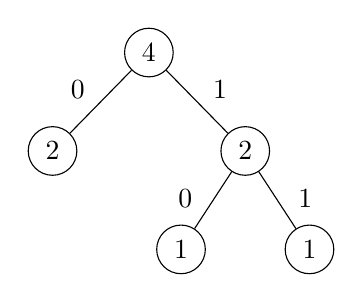
\begin{tikzpicture}[every tree node/.style={draw,circle},
  level distance=1.25cm,sibling distance=1cm,
  edge from parent path={(\tikzparentnode) -- (\tikzchildnode)}]
\Tree
[.4
   \edge node[auto=right,pos=.6] {$0$};
   [.2 ]
   \edge node[auto=left,pos=.6] {$1$};
   [.2 
       \edge node[auto=right,pos=.8] {$0$};
       [.1 ]
       \edge node[auto=left,pos=.8] {$1$};
       [.1 ]
       ]
]
\end{tikzpicture}
\\[10pt]
Assume it is true for k-1, then for k, we have $f_n....f_k+1$ and $s_k$ in the list, since $s_k = f_{k+2}-1$ then the smallest two number will be $f_k+1$ and$s_k$ then we combine them together. And construct a new node.
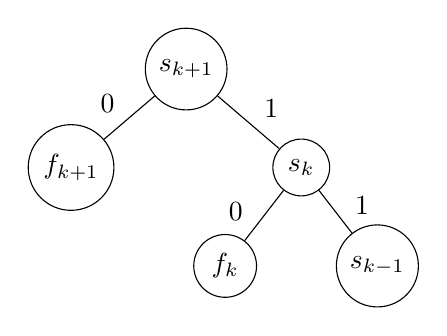
\begin{tikzpicture}[every tree node/.style={draw,circle},
  level distance=1.25cm,sibling distance=1cm,
  edge from parent path={(\tikzparentnode) -- (\tikzchildnode)}]
\Tree
[.$s_{k+1}$
   \edge node[auto=right,pos=.6] {$0$};
   [.$f_{k+1}$ ]
   \edge node[auto=left,pos=.6] {$1$};
   [.$s_k$ 
       \edge node[auto=right,pos=.8] {$0$};
       [.$f_k$ ]
       \edge node[auto=left,pos=.8] {$1$};
       [.$s_{k-1}$ ]
       ]
]
\end{tikzpicture}\\[10pt]
Then it is true that my code is the optimal.
\end{solution}
\fi

\end{itemize}
\newproblem{Cable Installation}{10 points}


\noindent
You operate a cable company and get $n$ request to install cable from
customers, whom we simply call $1,\ldots, n$. Each customer ordered a
different package, so that customer $i$ pays price $p[i]$ per each day
of service. Unfortunately, you can only do one installation per day,
so you must choose some order according to which you will do the $n$
installations. Namely, you must choose a permutation $\pi$ from
$\{1\ldots n\}$ to $\{1\ldots n\}$, so that the first day you go to
customer $\pi(1)$, the second --- to $\pi(2)$, etc., until you finish
at customer $\pi(n)$ at day number $n$. Since after day number $n$ you
get consistent revenue $p_1+\ldots+p_n$ per day irrespective of the
order of installations, your objective is to find the order $\pi$
maximizing the revenue during the first $n$ days, which equals to
$$Revenue(\pi) = p[\pi(1)]\cdot n + p[\pi(2)]\cdot (n-1) + \ldots +
p[\pi(n)]\cdot 1$$ Design a greedy algorithm for this problem. Use the
{\em Greedy Stays Ahead} principle to argue that your solution is
correct. You will begin by clearly defining $R_\pi(i)$ for any presumed solution $\pi$ 
and for $i=1,\ldots,n$.
Now let $\rho(n)$ be any other optimal ordering of installations, 
and let $\pi(n)$ be the ordering generated by your algorithm. You will 
then show that $R_\pi(i)\geq R_\rho(i)$ for all $i=1,\ldots,n$ \\
\hint{Split the revenue for the first $i$ days as the revenue for day
$1$ plus that for day $2$, $\ldots$ plus that for day $i$. Argue that
greedy gives a ``pretty good'' revenue for every specific day.}

\ifnum\me<2
\begin{solution}   
  \begin{code}
    1 \> {\sc Maximize-Revenue}$(P)$\\
    2 \> \> heap = Build-max-heap(P)\\
    3 \> \> revenue = 0, n=P.length\\
    4 \> \> while heap$!=null$\\
    5 \> \> \>revenue = revenue+heap.extractmax$\cdot$ n\\
    6 \> \> \>n=n-1\\
    7 \> \> \Return $revenue$
    \end{code}
    In word, i will choose $\pi(1)$ to be the index whose P[$\pi(1)$] is the maximum of all P[n], then $\pi(2)$ to be the second maximum one and so on.\\[10pt]
    $R_\pi(i) = P_{1-max}\cdot i+P_{2-max}\cdot (i-1)+P_{3-max}\cdot (i-2)+P_{i-max}\cdot 1$ here $P_{i-max}$ means the ith maximum value in P.\\[10pt]
    The revenue for day i is denoted as $DR_i$, then $R_\pi(i)$ can be written as $DR_1+DR_2+...+DR_i$ here $DR_i = p[\pi(1)]+p[\pi(2)]+...+p[\pi(i)]$\\[10pt]
    \textbf{proof by induction}\\[10pt]
    \textbf{basecase:} i=1, then $R_\pi(1) = P_{1-max}$ since it is the maximum value in p, then what ever $R_\rho(1)$ choose from p, it must be smaller than or equal to $P_{1-max}$, then $R_\pi(1) \ge R_\rho(1)$\\[10pt]
    \textbf{Recursive part:} assume it is true that  $R_\pi(i-1) \ge R_\rho(i-1)$, then for day i , the $DR_i = p[\pi(1)]+p[\pi(2)]+...+p[\pi(i)]$. For Strategy $\pi$ our $DR_i = P_{1-max}+P_{2-max}+...+P_{i-max}$,
     for Strategy $\rho$ this $DR_i = p[\pi(1)]+p[\pi(2)]+...+p[\pi(i)]$. Since our Strategy here takes the sum of 1-max to i-max value from p, then this sum should be greater than or equal to the sum of any i numbers, which is taken from p.
     Then in this way, we get $$R_\pi(i)=R_\pi(i-1)+DR_{\pi i} \ge R_\rho(i-1)+DR_{\rho i} = R_\rho(i)$$\\[10pt]
     Then for each day i our greedy strategy $\pi$ always have a better performance than other optimal solutions.



\end{solution}
\fi


\newproblem{Synchronizing the Clock}{18 points}
Consider the application of group messaging. It is not uncommon to utilize 
a tree, especially a binary tree, as a way to model this group. By using a binary tree,
one can have each of the group member to be the leaf and the server to be at 
the root of the tree. For purposes of this question, let us 
assume that we have a complete balanced binary tree with $n$ leaves where
$n$ is a power of two. Further, each non-root node $v$ contains $v.weight$ which
is the measure of the delay along the edge connecting $v$ to its parent $v.parent$.
From time to time, the server sends a synchronization message
announcing the time. The goal is to assign $v.newweight\geq v.weight$ so as to minimize
sum of all new weights and achieve synchronization at the leaves, i.e, all
the leaves get the message at the same time. 

We will use Greedy Strategy to solve this problem. We will begin by solving 
it for a toy problem. 
\begin{itemize}
	\item [(a)] (2 points) Consider the following binary tree. 
	\begin{center}
	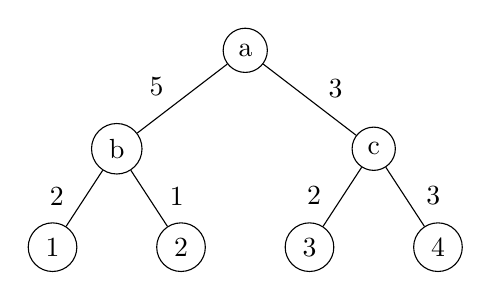
\begin{tikzpicture}[every tree node/.style={draw,circle},
   level distance=1.25cm,sibling distance=1cm,
   edge from parent path={(\tikzparentnode) -- (\tikzchildnode)}]
\Tree
[.a
    \edge node[auto=right,pos=.6] {$5$};
    [.b 
       \edge node[auto=right,pos=.8] {$2$};
       [.1 ]
       \edge node[auto=left,pos=.8] {$1$};
       [.2 ]
        ]
    \edge node[auto=left,pos=.6] {$3$};
    [.c 
        \edge node[auto=right,pos=.8] {$2$};
        [.3 ]
        \edge node[auto=left,pos=.8] {$3$};
        [.4 ]
        ]
]
\end{tikzpicture}
\end{center}
Clearly, the leaves receive their messages at different time. Modify
the edge weights to make sure that the leaves are synchronized, while
minimizing the sum of the total edge length. 
\ifnum\me<2
\begin{solution}   
	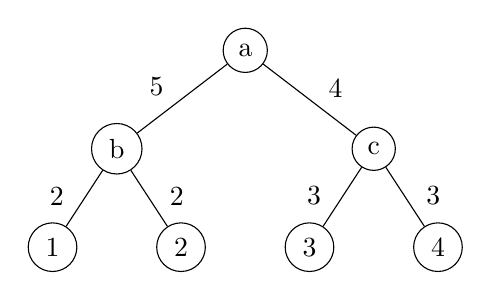
\begin{tikzpicture}[every tree node/.style={draw,circle},
    level distance=1.25cm,sibling distance=1cm,
    edge from parent path={(\tikzparentnode) -- (\tikzchildnode)}]
 \Tree
 [.a
     \edge node[auto=right,pos=.6] {$5$};
     [.b 
        \edge node[auto=right,pos=.8] {$2$};
        [.1 ]
        \edge node[auto=left,pos=.8] {$2$};
        [.2 ]
         ]
     \edge node[auto=left,pos=.6] {$4$};
     [.c 
         \edge node[auto=right,pos=.8] {$3$};
         [.3 ]
         \edge node[auto=left,pos=.8] {$3$};
         [.4 ]
         ]
 ]
 \end{tikzpicture}
\end{solution}
\fi
\item[(b)] (3 points) Consider a subtree rooted at $v$. Let $v.d$ be the 
length of the longest path from the leaf in this subtree to $v$. 
Clearly, $v.d=0$ for a leaf node. 
Devise a {\em recursive} algorithm 
to update this value for the binary tree. 
You are given a skeleton
pseudocode. Complete the pseudocode by filling in the blanks. 
Argue that your algorithm has a runtime of $O(n)$ using a suitable
recurrence equation. \hint{Choose a suitable tree-walk to complete this algorithm.} 
\begin{code}
1 \> {\sc Update-d}$(v)$\\
2 \> \> \If $\ldots\ldots\ldots\ldots\ldots=\Nil$ \Then $\Return \ldots\ldots\ldots\ldots\ldots$\\
3 \> \> $valuel=\ldots\ldots\ldots\ldots\ldots$\\
4 \> \> $valuer=\ldots\ldots\ldots\ldots\ldots$\\
5 \> \> $v.d=\ldots\ldots\ldots\ldots\ldots$\\
6 \> \> \Return $v.d$
\end{code}

\ifnum\me<2
\begin{solution}   
  \begin{code}
    1 \> {\sc Update-d}$(v)$\\
    2 \> \> \If v.left and v.right=\Nil$ \Then $\Return 0\\
    3 \> \> $valuel$=Update-d(v.left)\\
    4 \> \> $valuer$=Update-d(v.right)\\
    5 \> \> $v.d=max(valuel+v.left.weight,valuer+v.right.weight)$\\
    6 \> \> \Return $v.d$
    \end{code}
\end{solution}
\fi
\item[(c)](3 points) Give a ``greedy'' formula for $v.newweight$ in terms
of various values of $w.d$ for appropriately chosen $w$'s by filling in the blanks.
Further, show that
$v.newweight\geq v.weight$. \hint{Note that you have a pointer $v.parent$. Also,
note that $v.weight$ is not needed once $v.d$ is computed.}

$$v.newweight=\ldots\ldots\ldots\ldots\ldots\ldots\ldots\ldots\ldots\ldots$$
\ifnum\me<2
\begin{solution}   
  $$v.newweight=v.parent.d-v.d$$
  Since v.parent.d = max(v.d+v.weight,v.parent.anotherchild.d+v.parent.anotherchild.weight)
  which means v.parent.d$\ge$ v.d+v.weight.\\[10pt]
  Then v.newweight $\ge v.parent.d-v.d = v.weight$

\end{solution}
\fi
\item[(d)] (3 points) Show that the assignment in Part (c) is a \emph{valid} solution. We will
prove something stronger: For every node $v$, if
you only look at the subtree rooted at $v$, all leaves get the message at the same
time using the above $v.newweight$ value. Further, this is equal to $v.d$. \hint{
Use induction on the depth of the node starting at leaves.}
\ifnum\me<2
\begin{solution}   
\textbf{Basecase}: The depth of the v is 0 which means this v is a leaf node , then it is abvious that its leaves will get message at the same time using v.newweight = 0, and it is equal to v.d\\[10pt]

\textbf{Induction}: Assume it is true for v whose depth is k-1, then for v whose depth is k. All leaves rooted at v.left will get message at the same time, and the time will be $v_{k-1left}$.d+$v_{k-1left}.newweight$
and the leaves rooted at v.right is the same. Then since $v.{k-1left}.newweight = v.d-v.left.d$ and $v.{k-1right}.newweight = v.d-v.right.d$ then all the leaves rooted at v.left will get message at the same time using time $v.d$ and it is the same with the right leaves.
Then all the leaves will get message at the same time with time v.d\\[10pt]
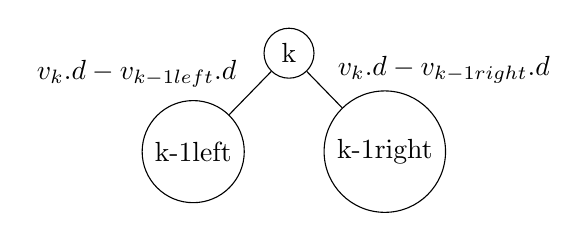
\begin{tikzpicture}[every tree node/.style={draw,circle},
  level distance=1.25cm,sibling distance=1cm,
  edge from parent path={(\tikzparentnode) -- (\tikzchildnode)}]
\Tree
[.k
   \edge node[auto=right,pos=.6] {$v_k.d-v_{k-1left}.d$};
   [.k-1left ]
   \edge node[auto=left,pos=.6] {$v_k.d-v_{k-1right}.d$};
   [.k-1right ]
]
\end{tikzpicture}
\end{solution}
\fi
\item[(e)](3 points) Use an exchange argument to show that in any optimal solution
$Z$, for every node $v$ either $v.left.newweight=v.left.weight$ or $v.right.newweight=v.right.weight$
\ifnum\me<2
\begin{solution}   INSERT YOUR SOLUTION HERE   \end{solution}
\fi
\item[(f)](1 point) Given $a,b,c,d\geq 0$, 
what is the only satisfying
assignment $a'\geq a,b'\geq b$ such that $a'+c=b'+d$ and either $a=a'$ or
$b'=b$.
\\

	$a'=\underline{~~~~~~~~~~~~~~~~~~~~~~~~~~},\ b'=\underline{~~~~~~~~~~~~~~~~~~~~~~~~~~}$

\ifnum\me<2
\begin{solution}   
  $a'=\underline{max(a+c,b+d)-c},\ b'=\underline{max(a+c,b+d)-d}$
\end{solution}
\fi
\item[(g)](3 points) Show that the algorithm that implements
the greedy formula from Part (c) is the only one satisfying the constraint of Part (e).\hint{Part (f) might be useful to help you solve this question.} 
\ifnum\me<2
\begin{solution}  	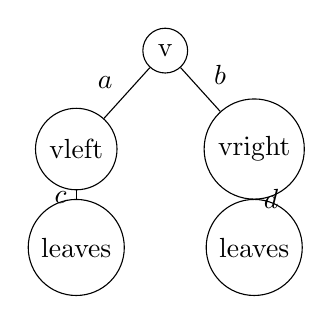
\begin{tikzpicture}[every tree node/.style={draw,circle},
  level distance=1.25cm,sibling distance=1cm,
  edge from parent path={(\tikzparentnode) -- (\tikzchildnode)}]
\Tree
[.v
   \edge node[auto=right,pos=.6] {$a$};
   [.vleft 
      \edge node[auto=right,pos=.8] {$c$};
      [.leaves ]
       ]
   \edge node[auto=left,pos=.6] {$b$};
   [.vright 
       \edge node[auto=right,pos=.8] {$d$};
       [.leaves ]
       ]
]
\end{tikzpicture} 
Assume that all the path from all the leaves rooted at the node vleft to vleft is c,the path from all the leaves rooted at the node vright to vright is d, ant the path from vleft to v is a,from vright to v is b
then inorder to make the leaves rooted at v to get message at the same time we should make a'+c = b'+d \\[10pt]
According to the problem f, we get that the only assignment of the new $a' = max(a+c,b+d)-c$ adn $b'=max(a+c,b+d)-d$\\[10pt]
Using a' as an example, $a' = vleft.newweight = max(a+c,b+d)-c$, $c = vleft.d$,$d=vright.d$ ,$a = vleft.weight$,$b = vright.weight$, then we get 
$$a' = vleft.newweight = max(vleft.weight+v.left.d,vright.weight+v.left.d)-vleft.d$$, according to the definition of v.d, it is the longest path from v to its leaves, then $$max(vleft.weight+v.left.d,vright.weight+v.left.d) = v.d$$
then we get $$a'vleft.newweight = v.d-v.left.d$$ which is the greedy formula from part c.
Then this formular is the only one satisfying the constraint of part(e).

\end{solution}
\fi
\end{itemize}
\end{document}


